%
% Encrypted Cloud Quantum Computation
%

\section{Encrypted cloud quantum computation} \label{sec:homo_blind} \index{Encrypted quantum computation}

\sectionby{Atul Mantri, Si-Hui Tan \& Peter Rohde}\index{Atul Mantri}

\dropcap{E}{xtremely} important to many high-performance data-processing applications is security, as proprietary or sensitive data may be being dealt with. To address this, there are two models for encrypted, outsourced quantum computation -- \textit{homomorphic encryption} \cite{bib:gentry2009fully, bib:van2010fully}\index{Homomorphic encryption} and \textit{blind quantum computation}\index{Blind quantum computation} \cite{bib:blind2, bib:broadbent2009universal, bib:barz2012demonstration, bib:PhysRevLett.108.200502, bib:Morimae3486, bib:Morimae5460, bib:Morimae5460}.

In both cases, Alice has secret data$^\copyright$, and wishes to not only ensure that an interceptor is unable to read it, but that even the server performing the computation isn't able to either -- she trusts no one. That is, she wishes the data to be processed in encrypted form, without first requiring decryption.

The difference between the two protocols lies in the treatment of algorithms:
\begin{itemize}
	\item Homomorphic encryption: Alice provides only the data, whereas Bob provides the processing and the algorithm it implements (which he would also like to keep to himself in general). When \textit{any} circuit is allowed, the protocol is said to be a \textit{fully homomorphic} encryption protocol (FHE). Otherwise, it is a \textit{somewhat-homomorphic} encryption protocol. Although homomorphic encryption protocols have been around for a few decades in the form of privacy homomorphisms \cite{bib:Rivest1978}, classical FHE has only been described very recently \cite{bib:gentry2009fully, bib:van2010fully}.
	\item Blind quantum computing: Alice provides both the algorithm \textit{and} the data, and wishes \textit{both} to remain secret to her. It is known that universal blind \textit{classical} computation is not possible, universal blind \textit{quantum} computation is.
\end{itemize}
Both of these seem like very challenging goals, yet significant developments have been made on both fronts in the quantum world, with efficient resource overheads associated with the encryption.

In the usual circuit model, blind quantum computation has been shown to be viable, and optimal bounds derived. Equivalently, such protocols have been described in the cluster state model (Sec.~\ref{sec:CSQC}). For universal computation, such protocols necessarily require classical interaction between the client and host. However, it was shown that in some restricted (i.e non-universal) models for optical quantum computation, specifically \textsc{BosonSampling}, quantum walks and coherent state passive linear optics, non-interactive, somewhat-homomorphic encryption may be implemented.

These encryption protocols induce a resource overhead in circuit size and number of qubits involved in the computation, with efficient scaling. They deliver (at least partially) information-theoretically secure (Sec.~\ref{sec:comp_vs_inf_th_sec}) data-hiding, enabling trustworthy outsourced processing of encrypted data, independent of the attack.

%
% Classical Computation 
%

\subsection{Classical computation} \index{Classical encrypted computation}
\comment{A universal QC can implement any classical algorithm. So QCs with homo/BQC give us the means by which to perform encrypted classical computations, bypassing limitations imposed by purely classical protocols.}
\comment{[Comment: The polynomial hierarchy is not contained in BQP. In fact, NP-complete problems are not contained in BQP.]}


To set the stage for our upcoming treatment of encrypted quantum computation protocols, we begin by reviewing recent developments in \textit{classical} homomorphic encryption, paying special interest to resource scaling and information-theoretic security.

\comment{The first FHE scheme was reported in Gentry's seminal paper \cite{bib:gentry2009fully}. He showed that if a homomorphic encryption scheme can evaluate its own decryption circuit, and also slightly augmented versions of it--a feature he calls {\it bootstrapping}, one can construct a FHE scheme from it. Then he constructed a somewhat homomorphic encryption protocol using ideal lattices, and via a clever transformation that decreases the complexity of its decryption circuit, showed that it is bootstrappable with respect to a universal set of gates. For a security parameter $\lambda$, Gentry's scheme has a $\widetilde{O}(\lambda^6)$ \footnote{The tilde in the big-O notation means that we are ignoring logarithmic factors.} bit bound on complexity for refreshing a ciphertext corresponding to a 1-bit plaintext \cite{bib:Gentrythesis}. This was subsequently reduced to $\widetilde{O}(\lambda^{3.5})$ \cite{bib:Damien2010}, $\widetilde{O}(\lambda)$ \cite{bib:Brakerski2011}, and ${\rm polylog (\lambda)}$ for any width-$\Omega(\lambda)$ circuit with $t$ gates \cite{bib:Craig2012}. }

\comment{A homomorphic encryption scheme is made up of four algorithms: a key generation algorithm, \textsc{KeyGen}, an encryption algorithm, \textsc{Encrypt}, an evaluation algorithm, \textsc{Evaluate}, and a decryption algorithm, \textsc{Decrypt}. The four algorithms have the following inputs and outputs:
\begin{itemize}
\item \textsc{KeyGen}$(\lambda)$: Takes as input a security parameter $\lambda$, and outputs a public-key $pk$, and a secret-key $sk$.
\item \textsc{Encrypt}$(pk, \pi_i)$: Takes as input $pk$, and a plaintext $\pi_i$. It outputs a ciphertext $\psi_i$.
\item \textsc{Evaluate}$(pk, C, \Psi)$: Takes as input $pk$, a permitted circuit $C$, and $\Psi=(\psi_1,\ldots, \psi_t)$. It outputs a ciphertext $\psi$.
\item \textsc{Decrypt}$(sk,\psi)$: Takes as input $sk$, and $\psi$ and outputs $C(\pi_1,\ldots, \pi_t)$.
\end{itemize}
The computational complexity of all these algorithms must be polynomial in $\lambda$, and in the case of the evaluation algorithm, polynomial in the size of the evaluation circuit $C$. The condition that \textsc{Decrypt}$(sk,\psi)$ outputs $C(\pi_1,\ldots, \pi_t)$ is a condition known as correctness which we require of the homomorphic encryption scheme. Furthermore, we also require ciphertext size and decryption time to be upper bounded by a function of the security parameter $\lambda$, independently of $C$. This last condition is known as compactness, and is necessary to exclude trivial schemes such as that which decrypts the ciphertexts first, and then apply $C$.}

\comment{The specifics of these algorithm vary from scheme to scheme, and as is in the case of FHE, usually contains sub-algorithms within them. Making FHE practical is an active area of research. Much of the problem lies in the bootstrapping required in Gentry's scheme, and some of these efforts lies in reducing the overhead required in bootstrapping or removing the need for bootstrapping entirely. Although there exists a plethora of FHE schemes, they are based mainly on two types of problems in lattice-based cryptography: the Shortest Vector Problem (SVP), and Learning with Errors (LWE) Problem. Gentry's original FHE was based on SVP, but over time, the schemes have moved towards a LWE approach because they offer lower overhead and are conceptually simpler . An overview of advances, and applications of homomorphic encryption can be found in a recent review \cite{bib:Halevi2017}.}

%
% Homomorphic Encryption
%

\subsubsection{Homomorphic encryption} \index{Homomorphic encryption}

\comment{To do!}
Yes
%
% Blind Computation
%

\subsubsection{Blind computation} \index{Blind quantum computation}

\comment{To do!}

%
% Cluster States
%

\subsection{Cluster states} \index{Encrypted quantum computation!Cluster states}

Most simply, if Alice has the limited quantum resources required to perform single-qubit measurements, and she knows the algorithm she wishes to implement, then by outsourcing just the cluster state preparation stage, whilst performing the single-qubit measurements herself, she can obviously obtain \textit{perfect} secrecy of both her data and her algorithm, since no one else is involved in the processing stage.

However, Alice may have access to no quantum resources whatsoever -- even single-qubit measurements -- requiring homomorphic encryption or blind quantum computing protocols that are native to the cluster state model. Both such protocols have been described, and in fact are conceptually more straightforward to understand in the cluster state formalism. 

\comment{To do}

\comment{Consider both BQC and homomorphic QC}

%
% Homomorphic Encryption
%

\subsubsection{Homomorphic encryption} \index{Homomorphic encryption}

\comment{To do!}

%
% Blind Quantum Computation
%

\subsubsection{Blind quantum computation} \index{Blind quantum computation}

\comment{To do!}

%
% Circuit Model
%

\subsection{Circuit model} \index{Encrypted quantum computation!Circuit model}

\comment{To do}

%
% Homomorphic Encryption
%

\subsubsection{Homomorphic encryption} \index{Homomorphic encryption}

\comment{To do!}

%
% Blind Quantum Computation
%

\subsubsection{Blind quantum computation} \index{Blind quantum computation}

\comment{To do!}

%
% Encryption Passive Optics
%

\subsection{Passive optics} \index{Encrypted quantum computation!Passive optics}

The previously discussed schemes for encrypted universal quantum computation required a degree of client/server interaction via classical communication. But perhaps there are some restricted (i.e non-universal) models for optical quantum computation, which lend themselves to passive, non-interactive encryption? And perhaps these restrictions simplify the physical resource requirements for encryption?

Let us formalise some reasonable requirements for such a scheme. We will require that:
\begin{itemize}
\item Alice's encoding (state preparation) and decoding (measurement) operations are separable, single-mode operations (i.e she has no quantum power of entanglement at her disposal).
\item Bob's computation is non-interactive, requiring no input from Alice beyond her input state.
\item Bob's computation is passive, requiring no intermediate measurement and feedforward.
\item Other than this, there are no constraints on the structure of the encoding/decoding operations, or the optical quantum computation being implemented (e.g it could encompass more than just linear optics).
\end{itemize}

We can express these requirements very generally and elegantly in terms of a commutation relation between the encoding ($\hat{E}$), decoding ($\hat{D}$), and computational ($\hat{U}$) operations. Furthermore, for the protocol to hide information, the plaintext basis states must not be invariant under the encoding operations. This enforces the criteria,
\index{Criteria for encrypted passive optics}
\begin{definition}[Encrypted passive optics] \label{def:enc_pass}
Let \mbox{$k=\{k_1,\dots,k_m\}$} be a partition of the key $k$ into sub-keys $\{k_i\}$, one associated with each mode $i$. Let $\hat{E}_i(k_i)$ and $\hat{D}_i(\tilde k_i)$ be the encoding and decoding operations for the $i$th mode. $\tilde k$ is a potentially transformed version of $k$, to accommodate that the encryption and decryption keys may be asymmetric, in which case we require that $\tilde{k}$ be efficiently computable from $k$. Let $\hat{U}$ be the computation. Then, separability of the encoding and decoding operations requires the following commutation relation to hold,
\begin{align} \label{eq:gen_pass_hom}
\hat{U} \left[\bigotimes_{i=1}^m\hat{E}_i(k_i)\right] = \left[\bigotimes_{i=1}^m\hat{D}^\dag_i(\tilde k_i)\right] \hat{U}.
\end{align}
For the protocol to hide information, the plaintext basis states must not be invariant under the encoding operations,
\begin{align}
\left[\bigotimes_{i=1}^m\hat{E}_i(k_i)\right]\ket\psi_\mathrm{plaintext} \neq \ket\psi_\mathrm{plaintext}.
\end{align}
The state observed by Bob is the mixture of Alice's plaintext over the complete set of encoding operations, implementing a quantum process $\mathcal{E}$, with Kraus operators $\hat{E}(k)$,
\begin{align} \label{eq:mix_over_enc_ops}
\hat\rho_\mathrm{encoded} &= \mathcal{E}(\ket\psi_\mathrm{plaintext}\bra\psi_\mathrm{plaintext}) \nonumber \\
&= \sum_k \hat{E}(k)\ket\psi_\mathrm{plaintext}\bra\psi_\mathrm{plaintext} \hat{E}^\dag(k),
\end{align}
where,
\begin{align}
\hat{E}(k) = \bigotimes_{i=1}^m\hat{E}_i(k_i).
\end{align}
To minimise Bob's chances of guessing Alice's state, we would like to maximise the von Neuman entropy of Bob's state. For \mbox{$S(\hat\rho_\mathrm{encoded})=0$} we have no secrecy, whereas for maximal \mbox{$S(\hat\rho_\mathrm{encoded})$} we have maximal secrecy (for the given plaintext basis state).
\end{definition} 

Intuitively, this simply says that a tensor product of single-mode encoding operations commutes through the passive computation to yield a (potentially different) tensor product of single-mode decoding operations. This way, Alice's operations are all separable, requiring no entangling gates (after all, if she had access to entangling gates she might be able to do quantum computations herself!). This relationship can be illustrated as shown in Fig.~\ref{fig:gen_pass_hom}.

Importantly, note that devising a scheme satisfying this commutation relation does not automatically imply that it is secure -- it merely enforces the separability of Alice's encoding and decoding operations. An actual security proof is far more demanding, and will be highly state-dependent.

\begin{figure}[!htbp]
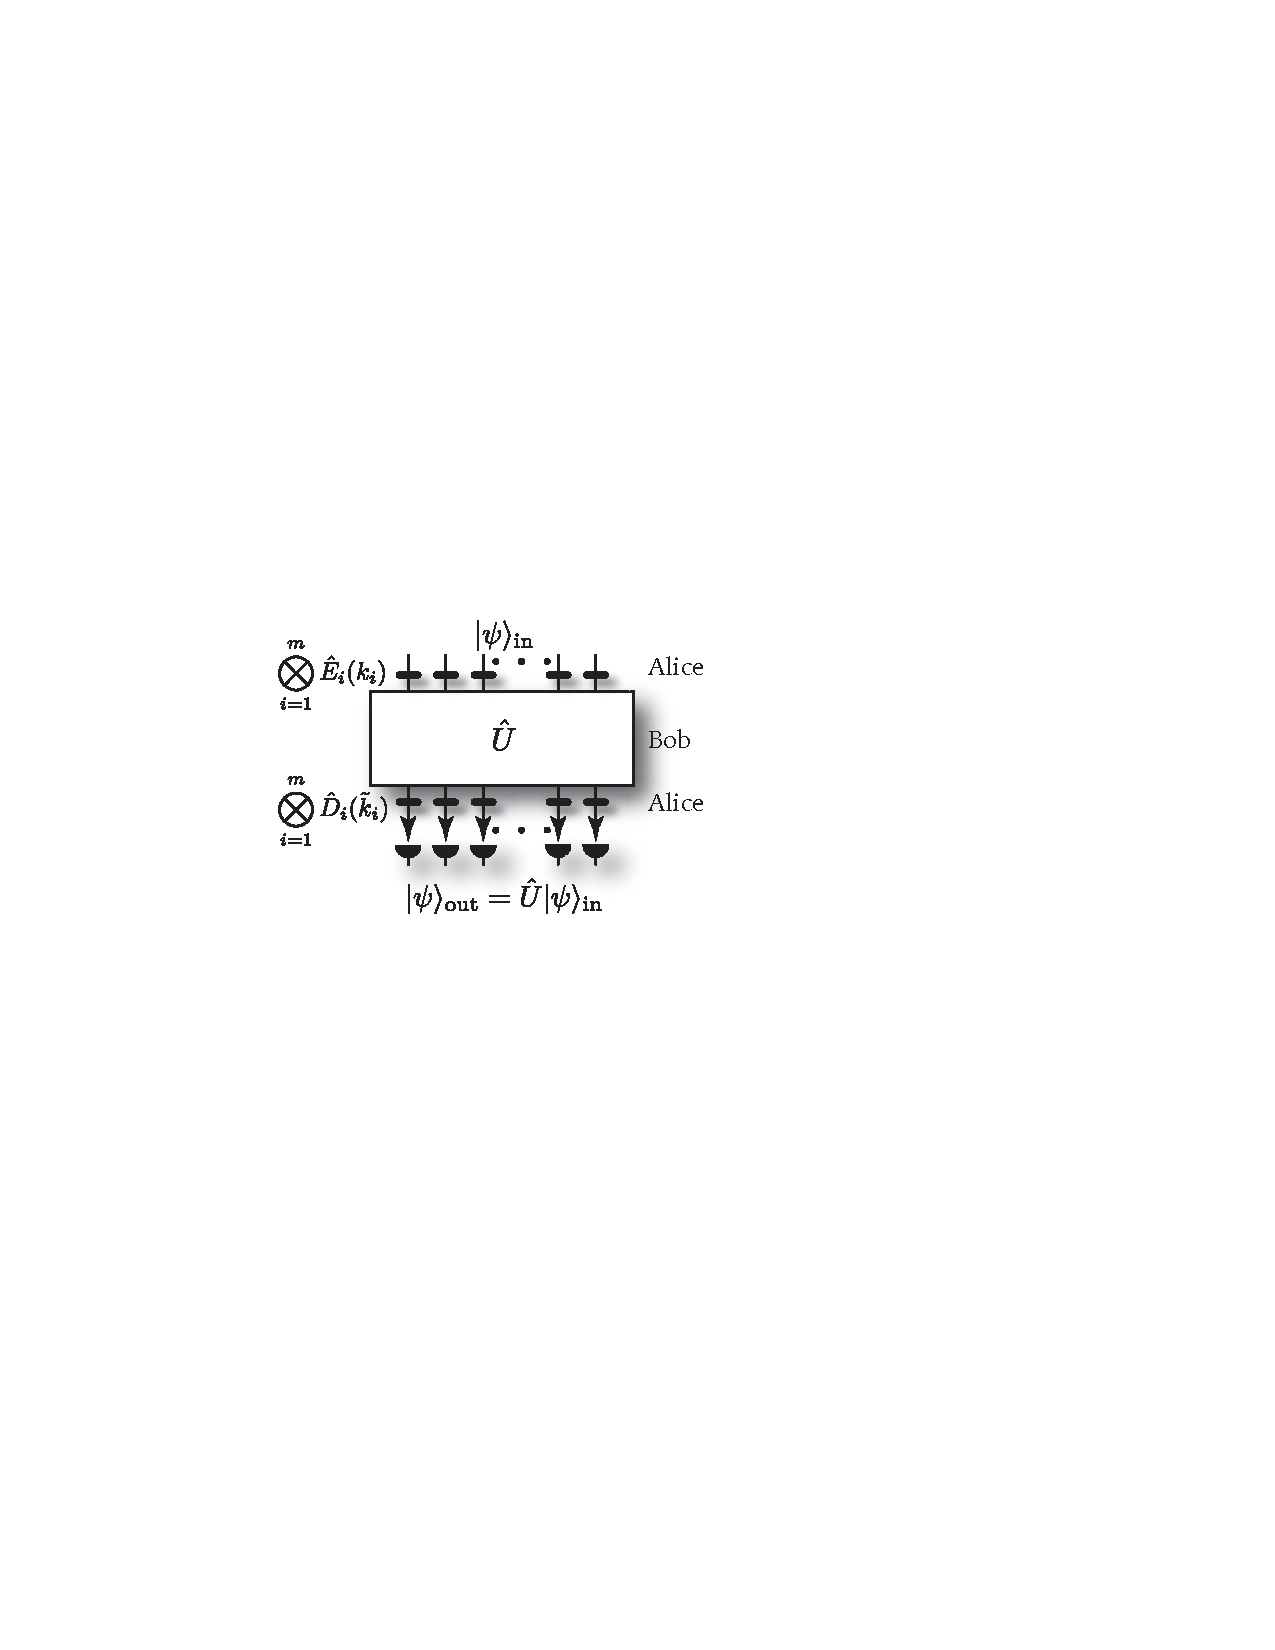
\includegraphics[clip=true, width=0.425\textwidth]{gen_pass_hom}
\captionspacefig \caption{General structure for the relationship between the encoding ($\hat{E}$), decoding ($\hat{D}$), and computational ($\hat{U}$) operations in a passive, non-interactive, optical quantum computation, where Alice is restricted to non-entangling, single-mode encoding and decoding operations.} \label{fig:gen_pass_hom}
\end{figure}

In the following sections we introduce non-interactive techniques for passive optical quantum computation based upon this general formalism. As encoding techniques compatible with the commutation relation from Eq.~(\ref{eq:gen_pass_hom}), we specifically introduce:
\begin{itemize}
\item \textit{Polarisation-key encoding} (Sec.~\ref{sec:phot_homo_enc}): a uniform random polarisation rotation is applied to each input mode, which we apply to photonic linear optics.\index{Polarisation!Key encoding}
\item \textit{Phase-key encoding} (Sec.~\ref{sec:homo_coherent_state}): a uniform random phase-shift is applied to each input mode, which we apply to the encryption of coherent states under evolution via linear optics and generalised non-linear phase-shift operations.\index{Phase!Key encoding}
\item \textit{Displacement-key encoding} (Sec.~\ref{sec:disp_key_enc}): an arbitrary configuration of random phase-space displacements is applied to the input modes, which in principle applies to any optical encoding.\index{Displacement-key encoding}
\end{itemize}
However, we leave it as an open question for future work to fully characterise the set of compatible encoding, decoding and computational operations, and to evaluate their security for different choices of input states.

%
% Polarisation-Key Encoding
%

\subsubsection{Polarisation-key encoding} \label{sec:phot_homo_enc} \index{Polarisation!Key encoding}

It was recently shown that processing photonic states using passive linear optics -- i.e \textsc{BosonSampling} or quantum walks (Secs.~\ref{sec:boson_sampling} \& \ref{sec:QW}) -- may be trivially homomorphically encrypted with the addition of additional photons and randomised polarisation rotations on the inputs \cite{bib:RohdeQWEnc12}, so-called \textit{polarisation-key encoding}. This encryption does not require any client/server interaction, remaining completely passive, yet achieving near optimal secrecy, hiding $O(\log (m))$ bits of information in an $m$-mode interferometer. Furthermore, it does not impose an overhead in circuit complexity, only in the number of input photons.

For $m$ modes, the resource requirements are:
\begin{enumerate}
\item $m$ single-photons -- one per input mode.
\item $m$ classically controlled wave-plates, able to implement arbitrary polarisation rotations.
\item $m$ polarisation filters.
\item $m$ photo-detectors.
\item An \mbox{$m\times m$} linear optics network.
\end{enumerate}
The full protocol is described in Alg.~\ref{alg:homo_LO} and shown in Fig.~\ref{fig:BS_homo}.

\begin{table}[!htbp]
\begin{mdframed}[innertopmargin=3pt, innerbottommargin=3pt, nobreak]
\texttt{
function PolarisationKeyEncoding($S$,$k$):
\begin{enumerate}
    \item Alice meditates upon, but needn't actually prepare the state,
    \begin{align}
    \ket\psi_\mathrm{number} = \ket{S_1,\dots,S_m},    
    \end{align}
    where,
    \begin{align}
S_i\in\{0,1\},
    \end{align}
is the photon-number of the $i$th mode.
   \item Alice makes the substitutions from the photon-number basis into the polarisation basis, 
   \begin{align}
   \ket{0}&\to\ket{H}, \nonumber \\
   \ket{1}&\to\ket{V},
   \end{align}
   to obtain $\ket\psi_\mathrm{pol}$, containing $m$ photons in total, one per mode.
   \item Alice chooses a random private-key $k$ as a real number from the uniform distribution,
   \begin{align}
    k\in(0,2\pi).
    \end{align}
    \item Alice prepares the encoded state by applying the same polarisation rotation (using wave-plates), of angle $k$, to each mode,
   \begin{align}
   \ket\psi_\mathrm{enc} = \hat{R}(k)^{\otimes m}\ket\psi_\mathrm{pol},
   \end{align}
   where,
   \begin{align}
   \hat{R}(\theta) = \begin{pmatrix}
\cos\theta & -\sin\theta \\
\sin\theta & \cos\theta
\end{pmatrix}.
   \end{align}
    \item Alice sends $\ket\psi_\mathrm{enc}$ to Bob.
    \item Bob applies processing using his linear optics computer, to obtain,
    \begin{align}
    \ket\psi_\mathrm{enc\,comp} = \hat{U} \ket\psi_\mathrm{enc}.
    \end{align}
    \item Bob returns $\ket\psi_\mathrm{enc\,comp}$ to Alice.
    \item Alice applies the inverse of the encoding operation,
    \begin{align}
    \ket\psi_\mathrm{comp} = \hat{R}(-k)^{\otimes m}\ket\psi_\mathrm{enc\,comp}.
    \end{align}
    \item Alice applies polarisation filters to $\ket\psi_\mathrm{comp}$, discarding horizontally polarised photons.
    \item The remaining vertically polarised state is Alice's unencrypted output of the computation.
    \item $\Box$
\end{enumerate}}
\end{mdframed}
\captionspacealg \caption{Protocol for implementing homomorphic encryption on photonic passive linear optics, using polarisation-key encoding.} \label{alg:homo_LO}
\end{table}

\begin{figure}[!htbp]
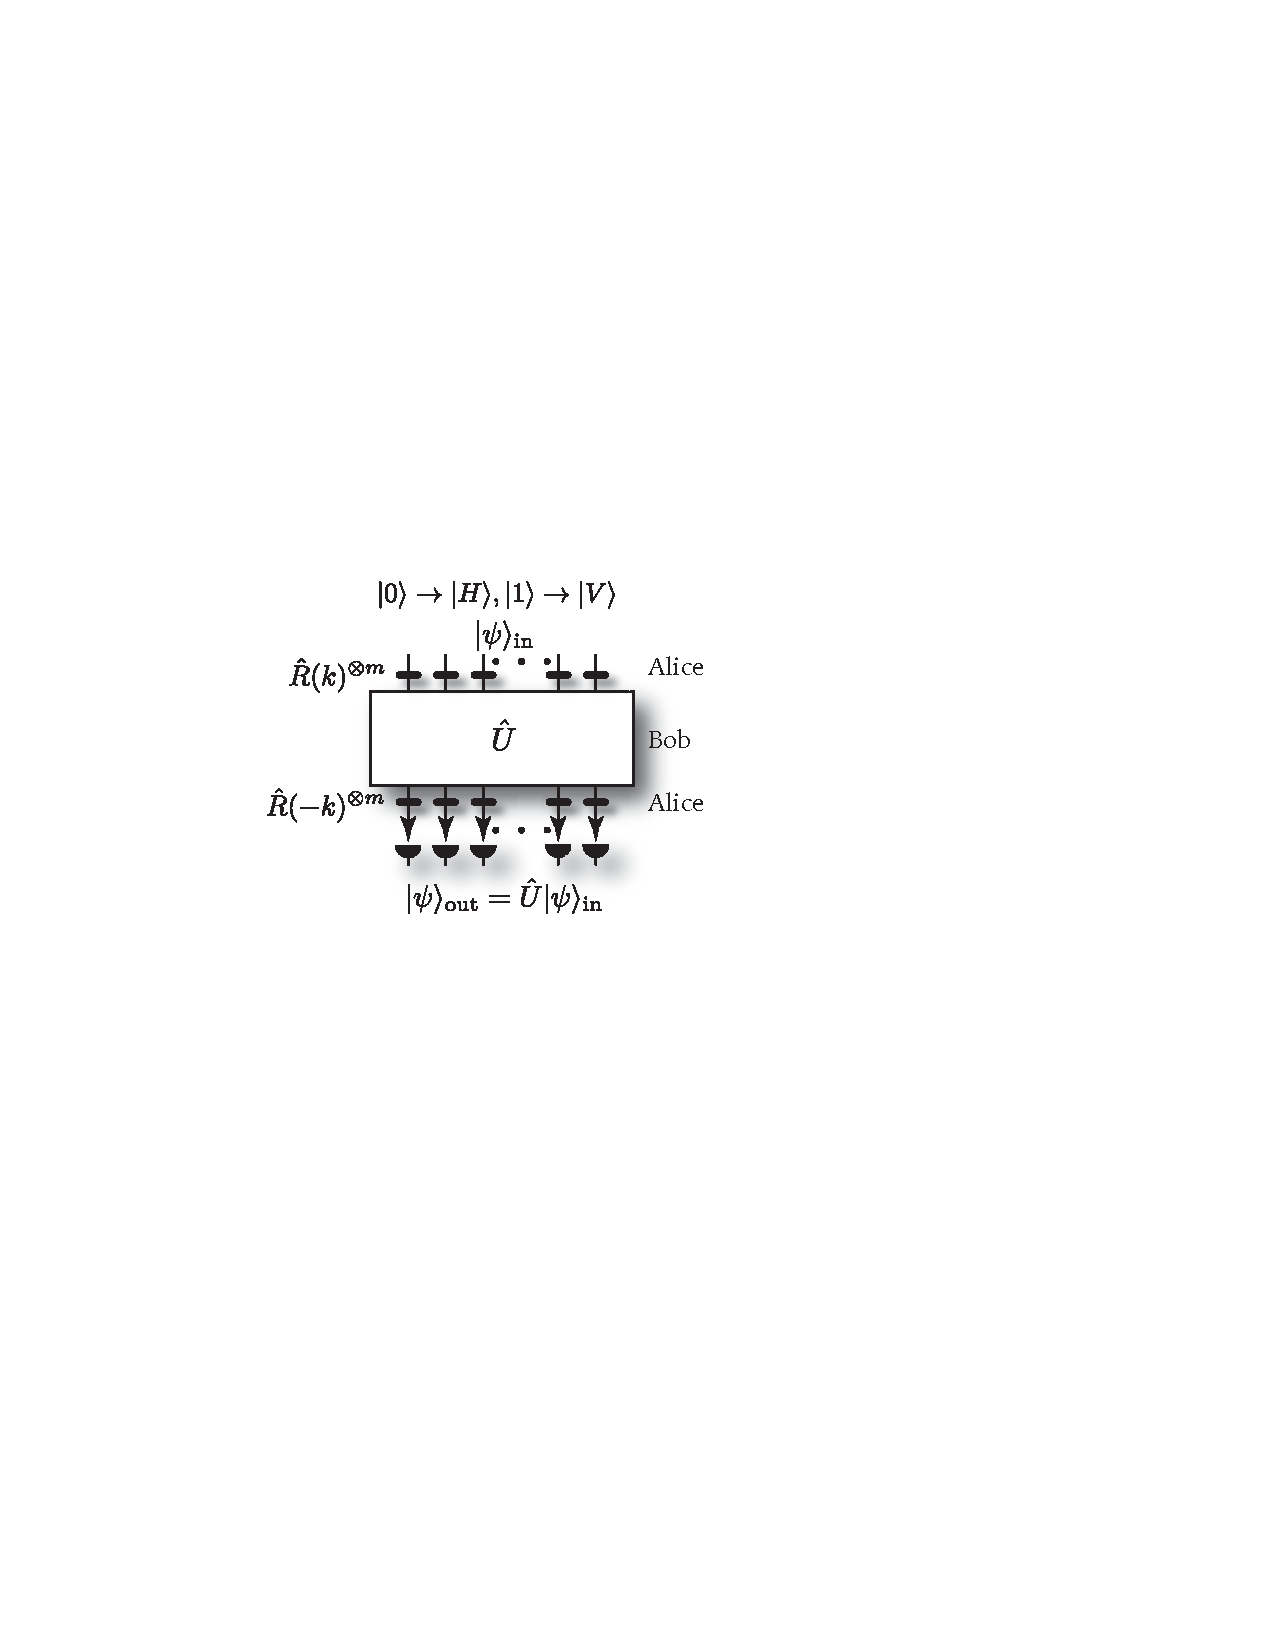
\includegraphics[clip=true, width=0.425\textwidth]{BS_homo}
\captionspacefig \caption{Protocol for implementing homomorphic encryption on photonic passive linear optics. Horizontal bars are wave-plates, implementing polarisation rotations $\hat{R}(\theta)$ -- the encryption and decryption operations performed by Alice. $\ket\psi_\mathrm{in}$ contains one photon per mode, polarisation-encoded such that vertically polarised photons belong to the desired computation, whilst the remaining horizontally polarised ones are dummies. The polarisation rotation angle, $k$, acts as Alice's private-key. The photo-detectors are polarisation-resolving, discarding all dummy horizontally polarised photons at the output. The algorithm is described in detail in Alg.~\ref{alg:homo_LO}.} \label{fig:BS_homo}
\end{figure}

The key idea here is that orthogonal polarisations do not interfere with one another under linear optics evolution. Thus, by inserting additional orthogonally polarised `dummy' photons, and applying uniform, random polarisation rotations, we can confuse any eavesdropper as to which photons belong to the computation, thereby hiding the secret data from them. Note that the encryption protocol does not affect the computation, since uniform polarisation rotations commute through linear optics circuits,
\begin{align} \label{eq:LO_key_commute}
\hat{R}(k)^{\otimes m} \hat{U} \hat{R}(-k)^{\otimes m} = \hat{R}(k)^{\otimes m} \hat{R}(-k)^{\otimes m} \hat{U} = \hat{U},
\end{align}
using the identity,
\begin{align}
\hat{R}(-k) = \hat{R}^\dag(k).	
\end{align}

Practically, $k$ could be chosen as some integer multiple of \mbox{$2\pi/d$}, where $d$ is the number of distinct keys, since an infinite precision key would be equivalent to an infinitely long key, were it represented as a bit-string. In this case, the information security of the protocol increases with $d$.

\cite{bib:RohdeQWEnc12} provided two relationships for the security of this protocol. First, the probability of Bob guessing Alice's input string approaches,
\begin{align}
P_\mathrm{guess} \leq \sqrt{\frac{8}{\pi m}},
\end{align}
for sufficiently large $m$ and $d$, which asymptotically (but unfortunately only polynomially\footnote{Note that an exponentially small bound is actually prohibited by no-go theorems for oblivious transfer and bit commitment \cite{bib:HKLo97, bib:SpekkensRudolphSecure}}) approaches 0.

Alternately, the mutual information between Alice and Bob, \mbox{$I(A;B)$}, can be upper-bounded using the Holevo quantity, $\chi$ \cite{bib:HolevoQuantity}. That is, \mbox{$I(A;B)\leq\chi$}. The Holevo quantity is defined as,\index{Holevo quantity}
\begin{align}
\chi = S(\hat\rho) - \sum_i p_i S(\hat\rho_i),
\end{align}
where,
\begin{align}
\hat\rho = \sum_i p_i \hat\rho_i,
\end{align}
and $S(\cdot)$ denotes the von Neuman entropy\index{von Neuman entropy} (Sec.~\ref{sec:channel_cap}). Here $\hat\rho_i$ are the individual codewords, in our case the set of all polarisation-encoded basis states, and $p_i$ are their respective probabilities, which are uniform here.

The upper-bound stipulated by the Holevo quantity is an information-theoretic bound\index{Information-theoretic!Bound}, which holds under \textit{any} choice of measurement bases by Bob. Thus, it is impossible for Bob to extract more information about Alice's state than allowed by this bound.

For this protocol the Holevo quantity scales with the number of modes as,
\begin{align}
\chi(m) = m - \frac{1}{2}\log_2\left(\frac{\pi e m}{2}\right) + O\left(\frac{1}{m}\right),
\end{align}
for sufficiently large $d$. Since there are $m$ bits of information in Alice's input state, this implies that the protocol hides at least,
\begin{align}
\frac{1}{2}\log_2\left(\frac{\pi e m}{2}\right) + O\left(\frac{1}{m}\right),
\end{align}
bits of information from Bob.

Furthermore, because a single computation requires Alice to perform only a single call to Bob's algorithm, which we treat as a black box, Alice gains minimum knowledge about Bob's secret algorithm, which is optimal for Bob.

Note that while we have considered linear optics in the above discussion, we could in fact expand the list of ingredients available to the computation to include anything generated by a Hamiltonian that commutes with polarisation rotations,
\begin{align}
[\hat{R}(\theta),\hat{H}]=0.
\end{align}
This could include, for example, polarisation-independent non-linear operations.

\comment{Discuss follow-up paper by Fitzsimons group on using other photonic degrees of freedom to enhance security.}

%
% Phase-Key Encoding
%

\subsubsection{Phase-key encoding} \label{sec:homo_coherent_state} \index{Phase!Key encoding}

As discussed in Sec.~\ref{sec:coherent_state_QC}, although not a \textit{quantum} computation, a system comprising multi-mode coherent state inputs, evolved via passive linear optics, implements simple matrix multiplication on the vector of input coherent state amplitudes,
\begin{align} \label{eq:betaUalpha}
\vec\beta = U\cdot\vec\alpha,
\end{align}
for input,
\begin{align}
\ket{\vec\alpha}=\ket{\alpha_1,\dots,\alpha_m},
\end{align}
and output,
\begin{align}
\ket{\vec\beta}=\ket{\beta_1,\dots,\beta_m}.
\end{align}
However, despite this being a classically efficient algorithm, it can experimentally be easily homomorphically encrypted with no computational resource overhead. This is in contrast to classical homomorphic encryption techniques, which incur a computational overhead.

The idea behind homomorphic encryption of coherent state linear optics is conceptually almost identical to the polarisation-space protocol for photonic linear optics (Sec.~\ref{sec:phot_homo_enc}). The key difference is that the random rotations are no longer applied in polarisation-space, but in phase-space as phase-rotations (\textit{phase-key encoding}). Specifically, the encryption/decryption operations are now given by the phase-shift operators, 
\begin{align}
\hat{R}(\phi) = \hat\Phi(\phi)=e^{-i\phi\hat{n}}.
\end{align}
Phase-shift operators acting on coherent states simply implement the transformation,
\begin{align}
\hat\Phi(\phi)\ket\alpha = \ket{e^{-i\phi}\alpha},
\end{align}
a simple rotation about the origin in phase-space.

Like polarisation rotations, uniform phase-shifts commute through linear optics networks, as per Eq.~(\ref{eq:LO_key_commute}), and thus the protocol has similar mathematical structure to the photonic case. Now the phase-shift angle, $\phi$, acts as Alice's private-key, which she applies uniformly to all input modes, applying inverse uniform phase-shifts after the computation to decrypt the state. The full algorithm is given in Alg.~\ref{alg:homo_coherent_LO}.

\begin{table}[!htbp]
\begin{mdframed}[innertopmargin=3pt, innerbottommargin=3pt, nobreak]
\texttt{
function PhaseKeyEncoding($\vec\alpha$,$k$):
\begin{enumerate}
    \item Alice prepares the input multi-mode coherent state,
    \begin{align}
    \ket\psi_\mathrm{in} = \ket{\vec\alpha} = \ket{\alpha_1,\dots,\alpha_m}.
    \end{align}
    \item Alice chooses a random private-key $k$ as a real number from the uniform distribution,
    \begin{align}
    k\in (0,2\pi).
    \end{align}
    \item Alice prepares the encoded state by applying the same phase-shift, of angle $k$, to each mode,
    \begin{align}
    \ket\psi_\mathrm{enc} = \hat\Phi(k)^{\otimes m}\ket\psi_\mathrm{in},
    \end{align}
    where,
    \begin{align}
    \hat\Phi(\phi) = e^{i\phi\hat{n}},
    \end{align}
    is the phase-shift operator.
    \item Alice sends $\ket\psi_\mathrm{enc}$ to Bob.
    \item Bob applies processing using his linear optics computer, to obtain,
    \begin{align}
    \ket\psi_\mathrm{enc\,comp} = \hat{U}\ket\psi_\mathrm{enc}.
    \end{align}
    \item Bob returns $\ket\psi_\mathrm{enc\,comp}$ to Alice.
    \item Alice applies the inverse of the encoding operation,
    \begin{align}
    \ket\psi_\mathrm{comp} = \hat\Phi(-k)^{\otimes m}\ket\psi_\mathrm{enc\,comp}.
    \end{align}
    \item The resulting state is,
    \begin{align}
    \ket\psi_\mathrm{comp} = \ket{\vec\beta} = \ket{\beta_1,\dots,\beta_m},
    \end{align}
    where,
    \begin{align}
    \vec\beta = U\cdot\vec\alpha.
    \end{align}
    \item $\Box$
\end{enumerate}}
\end{mdframed}
\captionspacealg \caption{Protocol for implementing homomorphic encryption on coherent state passive linear optics, using phase-key encoding.} \label{alg:homo_coherent_LO}
\end{table}

In fact, this encryption technique applies to more than just linear optics, but extends to also include generalised non-linear phase-shift operations, generated by Hamiltonians that are polynomials in the photon-number operators,
\begin{align}
\hat{H} = O(\mathrm{poly}(\hat{n}_1,\dots,\hat{n}_m)),
\end{align}
where $\hat{n}_i$ is the photon-number operator for the $i$th mode\index{Photon-number!Operators}. This observation follows trivially from the observation that the phase-shift encoding operations (which are generated by Hamiltonians linear in the photon-number operators) commute with any polynomial in the photon-number operators,
\begin{align}
[\hat{n}_i,\mathrm{poly}(\hat{n}_1,\dots,\hat{n}_m)] = 0\,\,\forall \, i.
\end{align}
This immediately significantly expands the class of operations available for the computation. In particular, while coherent states remain separable under linear optics evolution, the introduction of non-linear phase-shift operations enables quantum entanglement, and presumably a more powerful class of computations than simple matrix multiplication. It is unclear to us, however, exactly what this class of computations actually is.

\cite{siHuiTan} evaluated the security of this protocol in the case where the basis states were restricted to the binary $\ket{\pm\alpha}$ states. Thus, each input mode encodes at most a single bit (zero bits for \mbox{$|\alpha|=0$}, approaching one bit for \mbox{$|\alpha|\to\infty$}). Rather than employing the mutual information, they resorted to the alternative approach of calculating the distinguishability of codewords under the trace distance (Sec.~\ref{sec:fid_metric}). This has a direct operational interpretation as the probability of Bob guessing Alice's state in the best case. If the basis codeword states observed by Bob are indistinguishable, they are effectively decorrelated from the plaintext basis states, preventing him from guessing Alice's plaintext state, whereas if they are distinguishable, he can.

Let $\vec{x}$ be the binary input string, and $\vec{0}$ be the special case of the all-zero string. Then, for unencrypted states, we have the trace distance,
\begin{align}
D_\mathrm{unenc} &= ||\hat\rho_{\vec{x}}-\hat\rho_{\vec{0}}||_\mathrm{tr} \nonumber \\
&= \sqrt{1-e^{-4\mathrm{wt}(\vec{x})|\alpha|^2}},
\end{align}
where $\mathrm{wt}(\vec{x})$ is the Hamming weight (number of 1s in the bit-string) of $\vec{x}$. On the other hand, for the encoded states, we have,
\begin{align}
D_\mathrm{enc} &= ||\mathcal{E}(\hat\rho_{\vec{x}})-\mathcal{E}(\hat\rho_{\vec{0}})||_\mathrm{tr} \\
&= \sum_{k=0}^{d-1} e^{-m|\alpha|^2}\frac{(m|\alpha|^2)^k}{k!}\sqrt{1-\left(\frac{m-2\mathrm{wt}(\vec{x})}{m}\right)^{2k}}, \nonumber
\end{align}
\comment{What's the limit as $d\to\infty$?} where $\mathcal{E}$ denotes the mixture over encoding operations observed by Bob, as per Eq.~(\ref{eq:mix_over_enc_ops}), and there are $d$ distinct keys. We also define the ratio between these two distances,
\begin{align}
R=\frac{D_\mathrm{enc}}{D_\mathrm{unenc}	},
\end{align}
as an indicator of data-hiding. \mbox{$R<1$} is indicative that information is hidden from Bob.

These relationships are illustrated in Figs.~\ref{fig:homo_coh_st_tr} \& \ref{fig:homo_coh_st_ratio}\footnote{Note that the distance between any arbitrary pair of codewords may be obtained by replacing $\mathrm{wt}(\cdot)$ with their Hamming distance (in the simple case where one of the codewords is the $\vec{0}$ bit-string, the Hamming weight and Hamming distance are equivalent).}. Clearly, the encoded basis states exhibit greater indistinguishability than the unencoded ones, demonstrating that information is hidden from Bob. The trace distance does not have the elegant interpretation of `number of bits hidden' that the mutual information does. Rather, it gives us the probability of Bob correctly guessing Alice's state, demonstrating the degree of partial hiding of information.

\if 1\doublecol
\begin{figure}[!htbp]
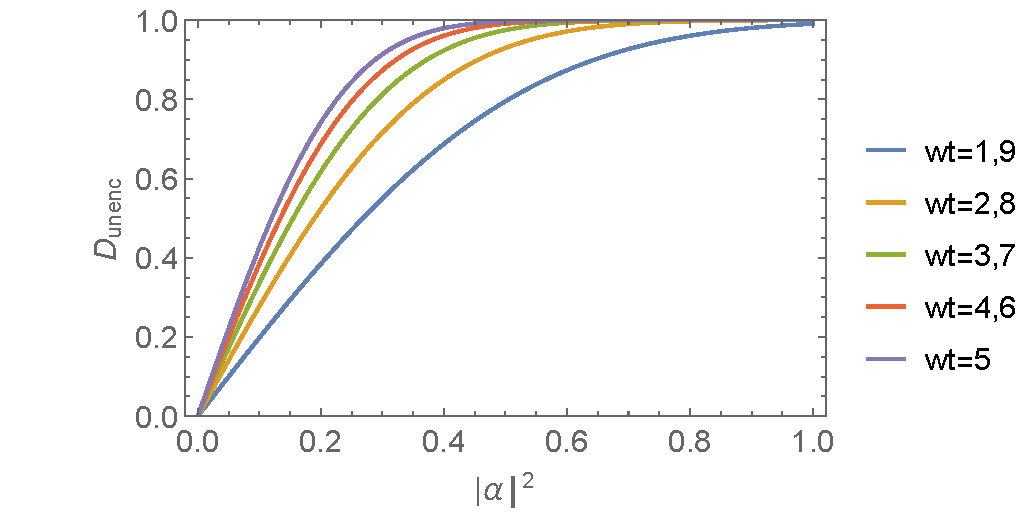
\includegraphics[clip=true, width=0.475\textwidth]{coherent_state_homo_unenc}\\
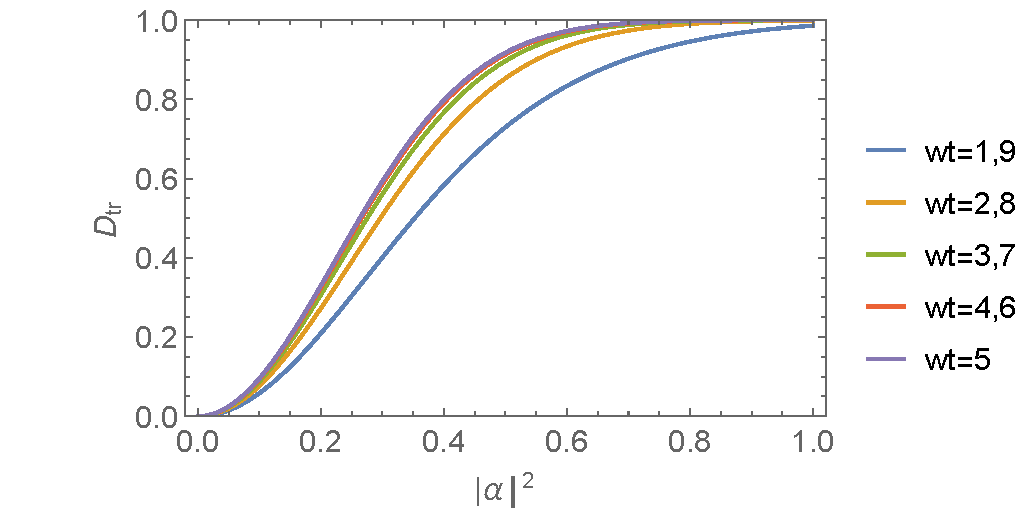
\includegraphics[clip=true, width=0.475\textwidth]{coherent_state_homo_enc}
\captionspacefig \caption{Trace distance between unencoded (top) and encoded (bottom) basis states for coherent state computation using phase-key encoding, with \mbox{$d=50$} keys and \mbox{$m=10$} modes. Each mode is inputted with one of two basis coherent states, \mbox{$\ket{\pm\alpha}$}. \mbox{$\mathrm{wt}(\vec{x})$} denotes the Hamming weight of bit-string $\vec{x}$. Two states are indistinguishable if their trace distance is 0, and distinguishable (orthogonal) if their trace distance is 1. Lower trace distance between encoded states implies a lower chance of Bob guessing Alice's plaintext input state.} \label{fig:homo_coh_st_tr}
\end{figure}
\else
\begin{figure*}[!htbp]
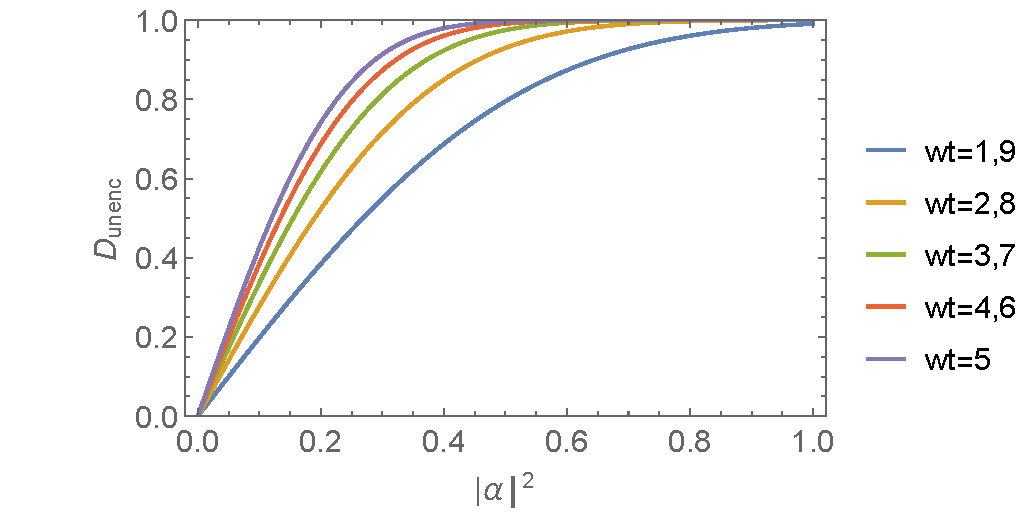
\includegraphics[clip=true, width=0.475\textwidth]{coherent_state_homo_unenc}
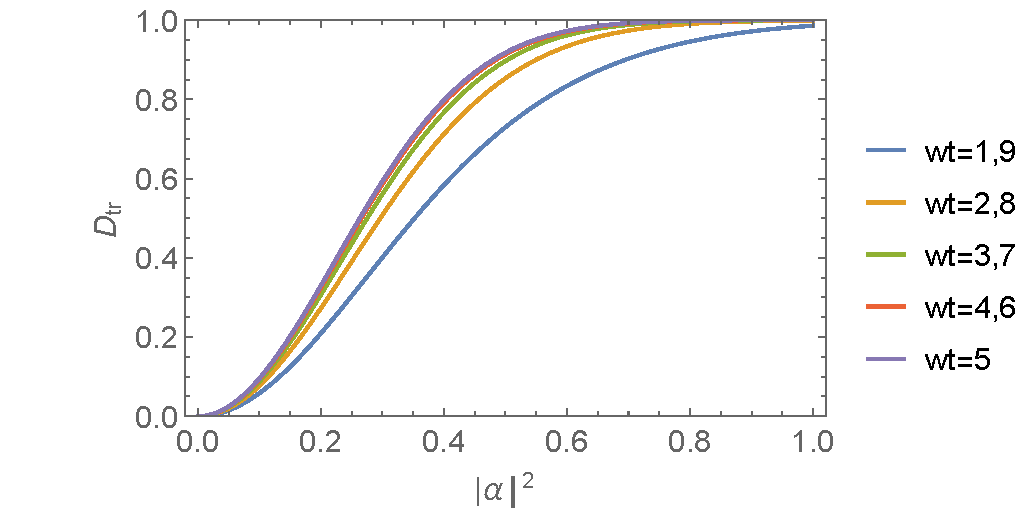
\includegraphics[clip=true, width=0.475\textwidth]{coherent_state_homo_enc}
\captionspacefig \caption{Trace distance between unencoded (top) and encoded (bottom) basis states for coherent state computation using phase-key encoding, with \mbox{$d=50$} keys and \mbox{$m=10$} modes. Each mode is inputted with one of two basis coherent states, \mbox{$\ket{\pm\alpha}$}. \mbox{$\mathrm{wt}(\vec{x})$} denotes the Hamming weight of bit-string $\vec{x}$. Two states are indistinguishable if their trace distance is 0, and distinguishable (orthogonal) if their trace distance is 1. Lower trace distance between encoded states implies a lower chance of Bob guessing Alice's plaintext input state.} \label{fig:homo_coh_st_tr}
\end{figure*}
\fi

\begin{figure}[!htbp]
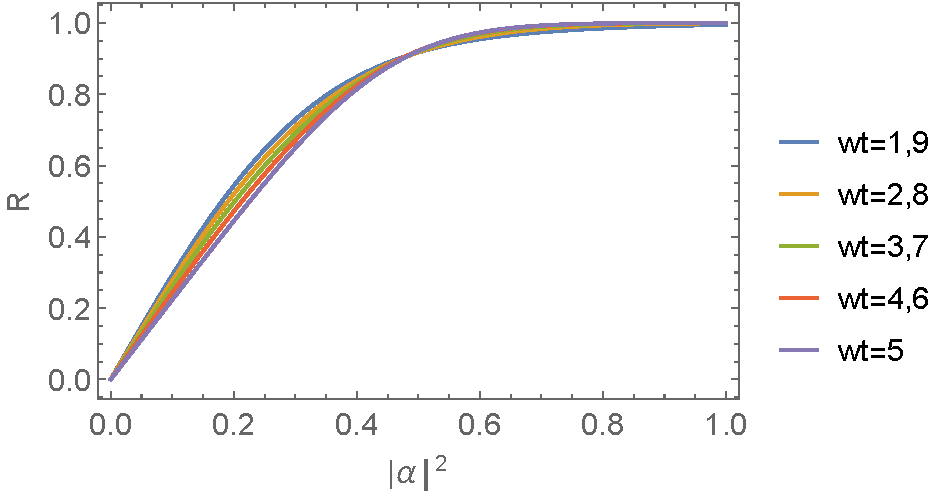
\includegraphics[clip=true, width=0.475\textwidth]{coherent_state_homo_ratio}
\captionspacefig \caption{Ratio of the trace distance between unencoded and encoded basis states for coherent state computation using phase-key encoding, with \mbox{$d=50$} keys and \mbox{$m=10$} modes. \mbox{$R<1$} implies information hiding from Bob.} \label{fig:homo_coh_st_ratio}
\end{figure}

It seems plausible that this approach to homomorphic encryption in phase-space could be extended to other quantum states of light. However, as is typically the case, performing entropic security proofs is notoriously difficult, and this remains an open problem. It should be noted, however, that this approach will definitely \textit{not} work for any class of input states which are invariant under phase-shifts. This explicitly rules out employing this technique for, for example, photon-number states, which have no phase.

This protocol demonstrates that a simple optical system is able to homomorphically encrypt the classical computation of matrix multiplication, as well as the more general operations of non-linear phase-shifts, without incurring the computational resource overhead imposed by conventional classical homomorphic encryption techniques.

\comment{Include figures for asymptotics against m and d.}

%
% Displacement-Key Encoding
%

\subsubsection{Displacement-key encoding} \label{sec:disp_key_enc} \index{Displacement-key encoding}

In the previous two sections we employed the encryption techniques of polarisation-key encoding and phase-key encoding. These are based on the observation that uniform polarisation- and phase-rotations commute through linear optics networks, as per Eq.~(\ref{eq:LO_key_commute}). Are there any other types of encoding operations that observe this property?

The other obvious candidate is \textit{displacement-key encoding}, whereby random displacements (not necessarily uniform across all modes) in phase-space (Sec.~\ref{sec:non_lin_opt}) form the encoding operations. Displacement operators exhibit the property that a tensor product of displacements commutes through linear optics circuits to yield a different combination of tensor products of displacements, where the displacement amplitudes obey the same relationship as for coherent states from Eq.~(\ref{eq:betaUalpha}). Specifically,
\begin{align}
\bigotimes_{i=1}^m \hat{D}_i(\alpha_i) \to \bigotimes_{j=1}^m \hat{D}_j(\beta_j),
\end{align}
where $\hat{D}_i(\alpha_i)$ is the displacement operator for the $i$th mode, with displacement amplitude $\alpha_i$, and the input and output displacement amplitudes are related according to,
\begin{align}
\vec\beta = \hat{U}\cdot\vec\alpha.
\end{align}

Based upon this observation, if the unitary $\hat{U}$ were known to Alice (i.e no secrecy for Bob's algorithm, unfortunately), she could efficiently encode and decode her state, since determining $\vec\beta$ from $\vec\alpha$ requires only classically-efficient matrix multiplication (residing in \textbf{P}\index{P}).

The algorithm for implementing displacement-key homomorphic encryption is shown in Alg.~\ref{alg:homo_disp_LO}.

\begin{table}[!htbp]
\begin{mdframed}[innertopmargin=3pt, innerbottommargin=3pt, nobreak]
\texttt{
function DisplacementKeyEncoding($\ket\psi$,$k$):
\begin{enumerate}
    \item Alice prepares the $m$-mode state $\ket\psi$.
    \item Alice chooses a set of independent complex displacement amplitudes as her private-key,
    \begin{align}
    k=\{\alpha_1,\dots,\alpha_m\}.
    \end{align}
    \item Alice applies the displacements to each mode, yielding her encrypted state,
    \begin{align}
    \ket\psi_\mathrm{enc} = \left[\bigotimes_{i=1}^m \hat{D}_i(\alpha_i)\right] \ket\psi,
    \end{align}
    where $\hat{D}_i(\alpha_i)$ is the displacement operator for the $i$th mode, with displacement amplitude $\alpha_i$.
    \item Alice sends the encrypted state to Bob.
    \item Bob applies the computation $\hat{U}$,
    \begin{align}
    \ket\psi_\mathrm{enc\, comp} = \hat{U}\ket\psi_\mathrm{enc}.
    \end{align}
    \item Bob returns the encrypted computed state to Alice.
    \item Alice calculates the inverse displacement amplitudes $\vec\beta$,
    \begin{align}
    \vec\beta = U\cdot\vec\alpha.
    \end{align}
    \item Alice applies the inverse displacements to each mode,
    \begin{align}
    \ket\psi_\mathrm{comp} &= \left[\bigotimes_{i=1}^m \hat{D}^\dag_i(\beta_i)\right] \ket\psi_\mathrm{enc\, comp} \nonumber \\
    &= \hat{U}\ket\psi,
    \end{align}
    \item $\ket\psi_\mathrm{comp}$ is the unencrypted computed output state.
    \item $\Box$
\end{enumerate}}
\end{mdframed}
\captionspacealg \caption{Protocol for implementing homomorphic encryption using displacement-key encoding.} \label{alg:homo_disp_LO}
\end{table}

Because performing the decoding operation requires solving the matrix multiplication problem to determine the decoding displacement amplitudes, this technique would obviously be inapplicable to encrypting, for example, coherent states, or other states which can be as efficiently classically simulated as matrix multiplication. Instead, it would only be relevant to linear optics sampling problems, which offer an exponential quantum speedup -- if performing the classical computation required for decryption is just as hard as performing the computation, Alice might as well do the computation herself!

Although currently no work has performed any security proofs for displacement-key encoding, this is a candidate approach that warrants future investigation, as displacements exhibit the right kind of commutation relations with linear optics that we desire. Furthermore, it is plausible that this approach might apply to a broad class of optical states, since, unlike phase-rotations, no optical states are invariant under non-zero displacements,
\begin{align}
\hat{D}(\alpha\neq 0)\ket\psi \neq \ket\psi\,\,\forall\,\ket\psi.
\end{align}

Intuitively we expect displacement-key encoding to potentially offer better security than phase-key encoding for two reasons:
\begin{enumerate}
\item Phase-keys are constrained in the range \mbox{$k=(0,2\pi)$}, whereas displacement amplitudes are effectively unbounded (nowadays we can make pretty big lasers!).
\item In phase-key encoding the encoding phase-rotation is uniform across all modes, yielding a mode-correlated encryption operation, which limits the entropy of Bob's perceived encoded state. On the other hand, for displacement-key encoding the encoding operations may be chosen independently for each mode, with no inter-mode correlations, potentially increasing the entropy of encoded codewords.
\end{enumerate}

\cite{???} presented a security analysis for displacement-key encoding applied to \textsc{BosonSampling}, which allows a direct side-by-side comparison with the polarisation-key encoded \textsc{BosonSampling} protocol discussed in Sec.~\ref{sec:phot_homo_enc}. As expected from the intuitive arguments presented above, it was found that displacement-key encoding can outperform polarisation- or phase-key encoding. In fact, in the limit of large upper-bounds on the displacement amplitudes, it was found that the scheme asymptotically perfectly hides Alice's information. That is, the mutual information between Alice and Bob is zero, as is the trace distance between codewords.

\begin{figure}[!htbp]
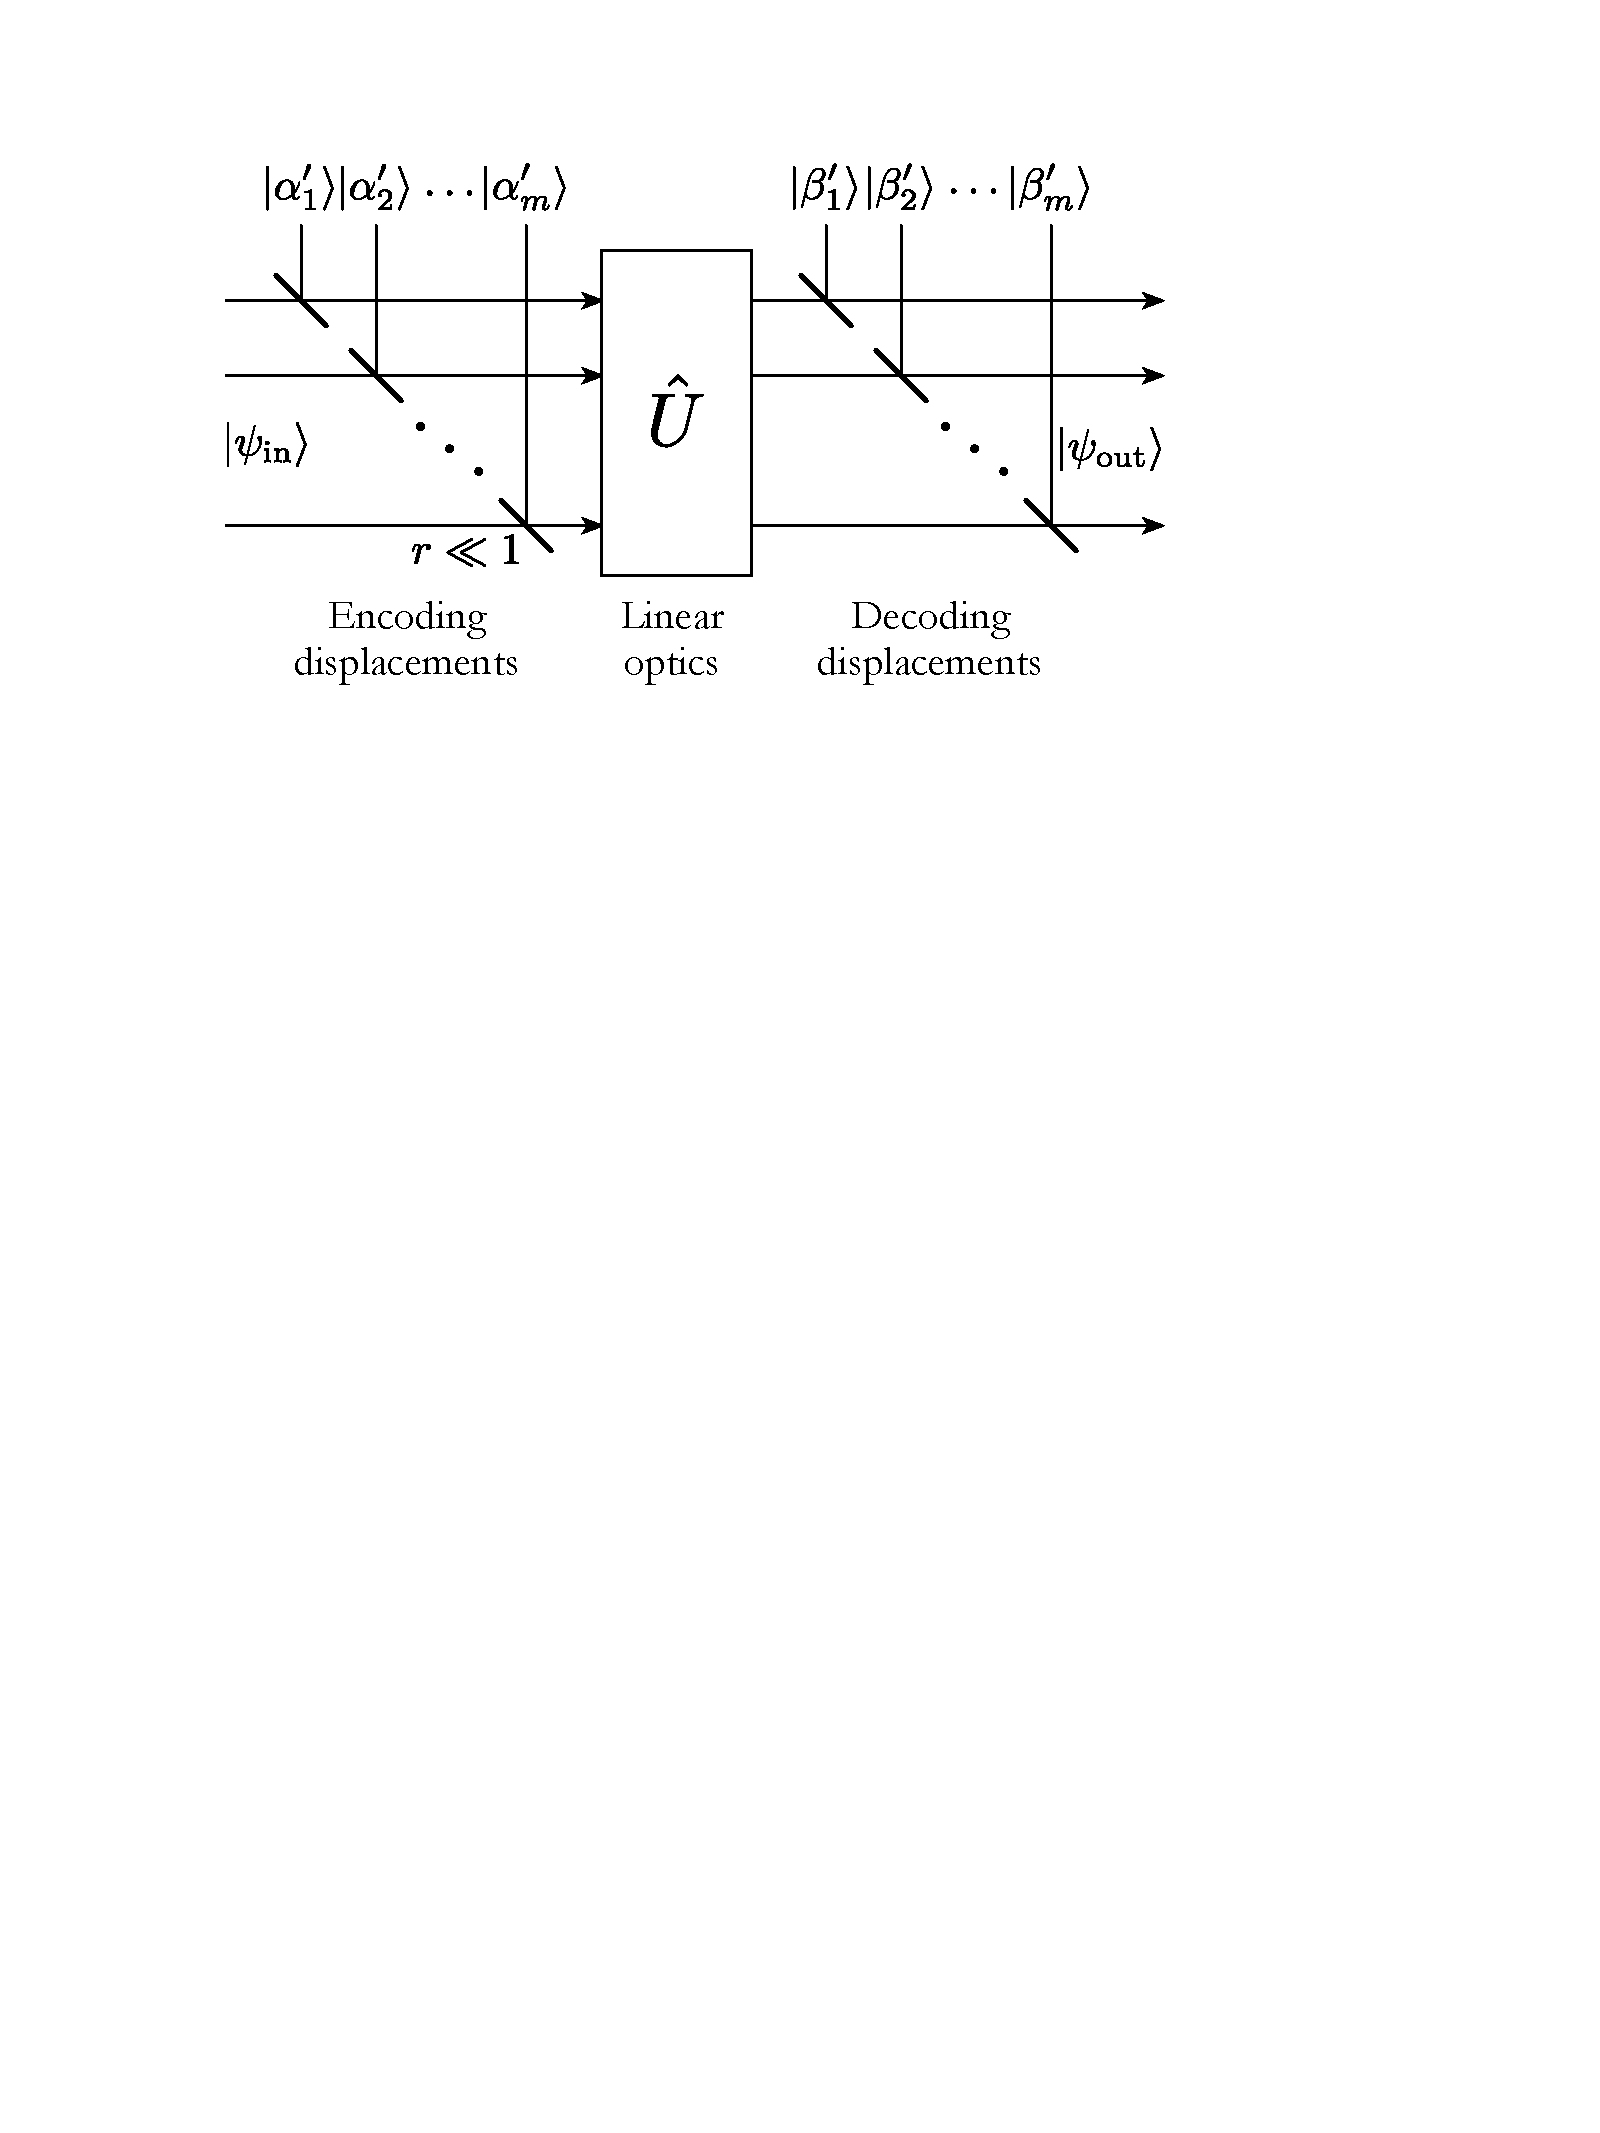
\includegraphics[clip=true, width=0.475\textwidth]{lo_displacement_homo}
\captionspacefig \caption{Circuit layout for displacement-key homomorphic encoding of passive linear optics, where \mbox{$\alpha_i'=\alpha_i/r$} and \mbox{$\beta_i'=\beta_i/r$}. Mixing the input modes with respective coherent states on a very low-reflectivity ($r$) beamsplitter implements the displacement operations. Following decoding, the output states is simply given by \mbox{$\ket{\psi_\mathrm{out}} = \hat{U}\ket{\psi_\mathrm{in}}$}, the computed input state.}\label{fig:lo_disp_key_circuit}	
\end{figure}

\comment{To do! Insert figures and equations.}

%
% One-Time Quantum Programs
%

\subsection{One-time quantum programs} \index{One-time quantum programs}

\comment{To do! Si-Hui?}

%
% Authentication
%

\subsection{Authentication} \index{Authentication}

\comment{To do}

\subsection{Digital signatures}

\subsection{Computing on shared sections}

